\documentclass[12pt]{article}
\usepackage{amsmath}
\usepackage{graphicx}
\usepackage{hyperref}
\usepackage{listings}
\usepackage{color}
\documentclass{article}
\usepackage{graphicx}


\title{Operating System Course Report - First Half of the Semester}
\author{B class}
\date{\today}

\begin{document}

\maketitle
\newpage

\tableofcontents
\newpage

\section{Introduction}
This report summarizes the topics covered during the first half of the Operating System course. It includes theoretical concepts, practical implementations, and assignments. The course focuses on the fundamentals of operating systems, including system architecture, process management, CPU scheduling, and deadlock handling.

\section{Course Overview}
\subsection{Objectives}
The main objectives of this course are:
\begin{itemize}
    \item To understand the basic components and architecture of a computer system.
    \item To learn process management, scheduling, and inter-process communication.
    \item To explore file systems, input/output management, and virtualization.
    \item To study the prevention and handling of deadlocks in operating systems.
\end{itemize}

\subsection{Course Structure}
The course is divided into two halves. This report focuses on the first half, which covers:
\begin{itemize}
    \item Basic Concepts and Components of Computer Systems
    \item System Performance and Metrics
    \item System Architecture of Computer Systems
    \item Process Description and Control
    \item Scheduling Algorithms
    \item Process Creation and Termination
    \item Introduction to Threads
    \item File Systems
    \item Input and Output Management
    \item Deadlock Introduction and Prevention
    \item User Interface Management
    \item Virtualization in Operating Systems
\end{itemize}

\section{Topics Covered}

\subsection{Basic Concepts and Components of Computer Systems}
This section explains the fundamental components that make up a computer system, including the CPU, memory, storage, and input/output devices.

\subsection{System Performance and Metrics}
This section introduces various system performance metrics used to measure the efficiency of a computer system, including throughput, response time, and utilization.

\subsection{System Architecture of Computer Systems}
Describes the architecture of modern computer systems, focusing on the interaction between hardware and the operating system.

\subsection{Process Description and Control}
Processes are a central concept in operating systems. This section covers:
\begin{itemize}
    \item Process states and state transitions
    \item Process control block (PCB)
    \item Context switching
\end{itemize}

\subsection{Scheduling Algorithms}
This section covers:
\begin{itemize}
    \item First-Come, First-Served (FCFS)
    \item Shortest Job Next (SJN)
    \item Round Robin (RR)
\end{itemize}
It explains how these algorithms are used to allocate CPU time to processes.

\subsection{Process Creation and Termination}
Details how processes are created and terminated by the operating system, including:
\begin{itemize}
    \item Process spawning
    \item Process termination conditions
\end{itemize}

\subsection{Introduction to Threads}
This section introduces the concept of threads and their relation to processes, covering:
\subsubsection{Kelebihan Multi-Threading}
\begin{itemize}
    \item\textbf{Responsive} 
    \par \hspace{2em} Multi-threading memungkinkan aplikasi tetap responsif bahkan jika sebagian thread terjebak dalam tugas yang lama. Sebagai contoh, dalam aplikasi GUI, thread utama tetap bisa merespons input pengguna sementara thread lain memproses tugas di latar belakang.
    \item\textbf{Resource Sharing}
    \par \hspace{2em} Dalam satu proses, semua thread dapat berbagi memori dan sumber daya (seperti file dan variabel). Ini membuat komunikasi antar-thread lebih efisien dibandingkan antar-proses, karena tidak memerlukan mekanisme komunikasi antar-proses yang kompleks.
    \item\textbf{Economics}
    \par \hspace{2em} Membuat dan mengelola thread lebih hemat sumber daya dibandingkan membuat proses baru, karena thread berbagi ruang memori dan sumber daya yang sama. Ini mengurangi biaya overhead yang dibutuhkan untuk alokasi memori dan waktu eksekusi.
    \item\textbf{Utilization}
    \par \hspace{2em} Multi-threading memaksimalkan penggunaan prosesor multi-core dengan memungkinkan berbagai thread berjalan secara paralel di core yang berbeda. Ini meningkatkan throughput aplikasi, sehingga meningkatkan kinerja keseluruhan pada sistem dengan banyak prosesor.
\end{itemize}

\subsubsection{Model Multi-Threading}
\begin{enumerate}
    \item\textbf{Many-To-One}
    \begin{figure}[h] 
        \centering 
        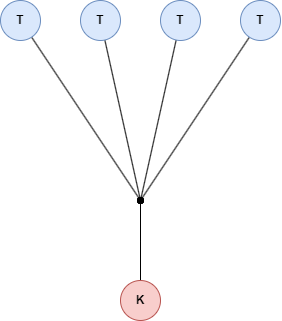
\includegraphics[width=0.5\textwidth]{asset/one to many.drawio.png} 
        \caption{many-to-one} 
        \label{fig:contoh} 
    \end{figure}
    \begin{itemize}
        \item\textbf{Definisi} 
        \par \hspace{2em} Many-to-One adalah model threading di mana banyak thread pengguna (user-level threads) dipetakan ke satu thread kernel. Dalam model ini, hanya ada satu thread kernel yang menangani eksekusi semua thread pengguna. Threading pada user space sepenuhnya dikelola oleh pustaka thread pengguna, dan kernel hanya mengenali satu thread aktif pada satu waktu.
        \item\textbf{Cara Kerja}
        \par \hspace{2em} Beberapa thread pengguna berjalan di dalam ruang alamat yang sama. Mereka saling berbagi data dan status. Kemudian, Hanya ada satu thread kernel yang menangani semua thread pengguna. Ketika sebuah thread pengguna menjalankan operasi blocking, seluruh thread dalam proses itu akan terblokir. Selain itu, Penjadwalan dilakukan sepenuhnya di tingkat pengguna. Thread pengguna melakukan manajemen dan penjadwalan sendiri tanpa intervensi kernel.
        \item\textbf{Contoh}
        \par \hspace{2em} Green threads pada implementasi awal Java.
    \end{itemize}
    \item\textbf{One-To-One} 
        \begin{figure}[h] 
            \centering 
            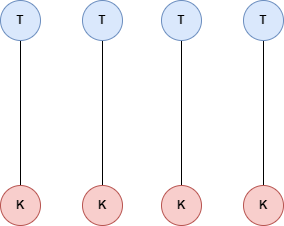
\includegraphics[width=0.5\textwidth]{asset/one to one.drawio.png} 
            \caption{one-to-one} 
            \label{fig:contoh} 
        \end{figure}
        \begin{itemize}
        \item\textbf{Definisi}
        \par \hspace{2em} One-to-One adalah model threading di mana setiap thread pengguna dipetakan langsung ke thread kernel. Setiap thread pengguna memiliki thread kernel yang terkait, sehingga kernel dapat mengelola eksekusi secara langsung. Dalam model ini, setiap thread yang dibuat pada level pengguna juga akan membuat thread pada kernel.
        \item\textbf{Cara Kerja}
        \par \hspace{2em} Setiap thread yang dibuat di ruang pengguna dikelola oleh kernel, dan masing-masing memiliki thread kernel tersendiri. Kemudian, Kernel dapat melakukan penjadwalan secara independen untuk setiap thread pengguna. Ini memungkinkan banyak thread dieksekusi secara bersamaan pada mesin multiprosesor. Selain itu, Penjadwalan dan manajemen dilakukan oleh kernel, sehingga kernel dapat menggunakan algoritma penjadwalan untuk memaksimalkan penggunaan CPU.
        \item\textbf{Contoh}
        \par \hspace{2em} Posix Threads (Pthreads) di Linux dan Windows.
    \end{itemize}
    \item\textbf{Many-To-Many}
        \begin{figure}[h] 
            \centering 
            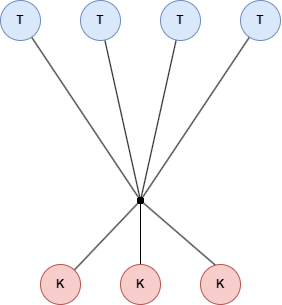
\includegraphics[width=0.5\textwidth]{asset/many to many.drawio.png} 
            \caption{many-to-many} 
            \label{fig:contoh} 
        \end{figure}
        \begin{itemize}
        \item\textbf{Definisi} 
        \par \hspace{2em} Many-to-Many adalah model threading di mana banyak thread pengguna dipetakan ke thread kernel yang lebih sedikit, tetapi tidak terbatas pada satu thread kernel saja. Thread pengguna dapat dijadwalkan dan dijalankan oleh beberapa thread kernel, memungkinkan concurrency yang lebih baik. Model ini mengizinkan thread pengguna untuk dijadwalkan ke thread kernel yang tersedia tanpa menciptakan ketergantungan satu-ke-satu atau satu-ke-banyak.
        \item\textbf{Cara Kerja}
        \par \hspace{2em} Banyak thread pengguna dapat berjalan secara bersamaan dan dapat dialokasikan ke thread kernel yang tersedia. Kemudian, Thread kernel bertindak sebagai mediator yang memungkinkan beberapa thread pengguna dieksekusi pada saat yang bersamaan, tergantung pada ketersediaan sumber daya kernel. Selain itu, Penjadwalan bisa dilakukan oleh kernel atau oleh pustaka thread, tergantung pada bagaimana sistem dirancang. Hal ini memungkinkan eksekusi thread yang lebih efisien.
        \item\textbf{Contoh}
        \par \hspace{2em} Beberapa sistem thread pada Solaris atau model thread hybrid.
    \end{itemize}
\end{enumerate}

\subsection{File Systems}
File systems provide a way for the operating system to store, retrieve, and manage data. This section explains:
\begin{itemize}
    \item File system structure
    \item File access methods
    \item Directory management
\end{itemize}

\subsection{Input and Output Management}
Input and output management is key for handling the interaction between the system and external devices. This section includes:
\begin{itemize}
    \item Device drivers
    \item I/O scheduling
\end{itemize}

\subsection{Deadlock Introduction and Prevention}
Explores the concept of deadlocks and methods for preventing them:
\begin{itemize}
    \item Deadlock conditions
    \item Deadlock prevention techniques
\end{itemize}

\subsection{User Interface Management}
This section discusses the role of the operating system in managing the user interface. Topics covered include:
\begin{itemize}
    \item Graphical User Interface (GUI)
    \item Command-Line Interface (CLI)
    \item Interaction between the user and the operating system
\end{itemize}

\subsection{Virtualization in Operating Systems}
Virtualization allows multiple operating systems to run concurrently on a single physical machine. This section explores:
\begin{itemize}
    \item Concept of virtualization
    \item Hypervisors and their types
    \item Benefits of virtualization in modern computing
\end{itemize}

\section{Assignments and Practical Work}
\subsection{Assignment 1: Process Scheduling}
Students were tasked with implementing various process scheduling algorithms (e.g., FCFS, SJN, and RR) and comparing their performance under different conditions.

\subsection{Assignment 2: Deadlock Handling}
In this assignment, students were asked to simulate different deadlock scenarios and explore various prevention methods.

\subsection{Assignment 3: Multithreading and Amdahl's Law}
This assignment involved designing a multithreading scenario to solve a computationally intensive problem. Students then applied **Amdahl's Law** to calculate the theoretical speedup of the program as the number of threads increased.
\subsubsection{Kelompok 7}

\begin{itemize}
    \item\textbf{Soal} 
    \par Desain sebuah skenario multithreading untuk menyelesaikan masalah komputasi intensif. Gunakan hukum Amdahl untuk menghitung kecepatan teoritis yang dihasilkan saat jumlah thread ditingkatkan.
    \item\textbf{Jawaban} 
    \begin{enumerate}
        \item Hukum Amdahl menghitung speedup maksimum suatu program berdasarkan porsi paralel dan sekuensial dari program tersebut.
        \item Speedup = 1 / (S + P/N), di mana S adalah porsi sekuensial, P adalah porsi paralel, dan N adalah jumlah thread.
    \end{enumerate} 

    \item\textbf{Implementasi Kode Python}
    \lstdefinestyle{mystyle}{
        basicstyle=\ttfamily\footnotesize,
        breakatwhitespace=false,         
        breaklines=true,                 
        captionpos=b,                    
        keepspaces=true,                                    
        numbersep=5pt,                  
        showspaces=false,                
        showstringspaces=false,
        showtabs=false,                  
        tabsize=2,
        frame=single                   
    }

        \lstset{style=mystyle}

    \begin{lstlisting}[language=Python, caption=Multithreading dan Amdahl's Law]
    import threading
    import time
    
    def intensive_task(n):
        result = 0
        for i in range(n):
            result += i ** 2
        return result
    
    # Skenario Multithreading
    def multithreaded_computation(num_threads, n):
        threads = []
        for i in range(num_threads):
            t = threading.Thread(target=intensive_task, args=(n//num_threads,))
            threads.append(t)
            t.start()
    
        for t in threads:
            t.join()
    
    # Hukum Amdahl
    def amdahls_law(s, p, n):
        return 1 / (s + (p / n))
    
    # Implementasi
    n = 1000000
    num_threads = 4
    sequential = 0.2
    parallel = 0.8
    
    start = time.time()
    multithreaded_computation(num_threads, n)
    end = time.time()
    
    print(f"Execution Time: {end - start}")
    print(f"Theoretical Speedup: {amdahls_law(sequential, parallel, num_threads)}")
    \end{lstlisting}

    \end{itemize}

\subsection{Assignment 4: Simple Command-Line Interface (CLI) for User Interface Management}
Students were tasked with creating a simple **CLI** for user interface management. The CLI should support basic commands such as file manipulation (creating, listing, and deleting files), process management, and system status reporting.

\subsection{Assignment 5: File System Access}
In this assignment, students implemented file system access routines, including:
\subsubsection{Kelompok 7}
\begin{itemize}
    \item\textbf{Soal} 
    \par Implementasikan rutin akses sistem file, termasuk: Pembuatan file, penghapusan file, Membaca file, menulis ke file dan Navigasi direktori serta pengelolaan izin file.
    \item\textbf{Implementasi Kode Python}
    \lstdefinestyle{mystyle}{
        basicstyle=\ttfamily\footnotesize,
        breakatwhitespace=false,         
        breaklines=true,                 
        captionpos=b,                    
        keepspaces=true,                                    
        numbersep=5pt,                  
        showspaces=false,                
        showstringspaces=false,
        showtabs=false,                  
        tabsize=2,
        frame=single                   
    }

        \lstset{style=mystyle}

    \begin{lstlisting}[language=Python, caption=File System Access]
    import os

    # Membuat dan menghapus file
    def create_file(filename="sisfo.txt"):
        with open(filename, 'w') as f:
            f.write("Initial content")
        print(f"File '{filename}' created.")
    
    def delete_file(filename="sisfo.txt"):
        if os.path.exists(filename):
            os.remove(filename)
            print(f"File '{filename}' deleted.")
        else:
            print(f"File '{filename}' not found.")
    
    # Membaca dan menulis file
    def write_to_file(filename="sisfo.txt", content=""):
        with open(filename, 'a') as f:
            f.write(content + "\n")
        print(f"Written to {filename}.")
    
    def read_file(filename="sisfo.txt"):
        if os.path.exists(filename):
            with open(filename, 'r') as f:
                print(f.read())
        else:
            print(f"File '{filename}' not found.")
    
    # Membuat direktori
    def navigate_directory(path):
        if os.path.exists(path):
            os.chdir(path)
            print(f"Changed directory to {path}")
        else:
            print(f"Directory '{path}' not found.")
    
    # Implementasi
    create_file()
    write_to_file(content="Hello World")
    read_file()
    delete_file()

    \end{lstlisting}

    \end{itemize}

\section{Conclusion}
The first half of the course introduced core operating system concepts, including process management, scheduling, multithreading, and file system access. These topics provided a foundation for more advanced topics to be covered in the second half of the course.

\begin{thebibliography}{9}
    \bibitem{anderson2000} Anderson, T. E., & Dahlin, M. (2000). \textit{User-level threads: The power of scheduling}. ACM Transactions on Computer Systems, 18(1), 70-110.
    \bibitem{silberschatz2018} Silberschatz, A., Galvin, P. B., & Gagne, G. (2018). \textit{Operating system concepts} (10th ed.). Wiley.
\end{thebibliography}


\end{document}